%=+=+=+=+=+=+=+=+=+=+=+=+=+=+=+=+=+=+=+=+=+=+=+=+=+=+=+=+=+=+=+=+=+=+=+=+=+=+=+=
%             _             _
%            | |           | |
%  _ __ ___  | |__    ___  | | ___   ___   _ __       ___   ___   _ __ ___
% | '_ ` _ \ | '_ \  / _ \ | |/ __| / _ \ | '_ \     / __| / _ \ | '_ ` _ \
% | | | | | || | | || (_) || |\__ \| (_) || | | | _ | (__ | (_) || | | | | |
% |_| |_| |_||_| |_| \___/ |_||___/ \___/ |_| |_|(_) \___| \___/ |_| |_| |_|
%
% Author: Mark H. Olson
% Website: https://mholson.com
% Github: https://github.com/mholson
%
% Created: 2021-06-09
%
% This is a template designed for International Baccaulaureate students who
% are looking to write an extended essary or internal assessment using LaTeX.
% It is based on the MAA monograph AMS/MAA textbook template
% (http://www.ams.org/arc/books/book-produce.html#maamono). Some modifications
% have been made to the original class files (maatext.cls and maabook.cls) to
% better meet the requirements of the International Baccaulaureate and these
% modifications are maintained at 
% (https://github.com/mholson/mhoTexmf/tree/main/texmf).  While
% the original tempalte was meant to be compiled using XeTeX, this tempalte has
% been designed to compile using pdflatex so that the cmbright font style
% can be applied to the document.
%=+=+=+=+=+=+=+=+=+=+=+=+=+=+=+=+=+=+=+=+=+=+=+=+=+=+=+=+=+=+=+=+=+=+=+=+=+=+=+=




%=-=-=-=-=-=-=-=-=-=-=-=-=-=-=-=-=-=-=-=-=-=-=-=-=-=-=-=-=-=-=-=-=-=-=-=-=-=-=-=
% SETUP :: main.tex 
%=-=-=-=-=-=-=-=-=-=-=-=-=-=-=-=-=-=-=-=-=-=-=-=-=-=-=-=-=-=-=-=-=-=-=-=-=-=-=-=
%
% Templates for text, math and figure elements are can be found at the end
% of this document ... below the \end{document} line.
%
%=-=-=-=-=-=-=-=-=-=-=-=-=-=-=-=-=-=-=-=-=-=-=-=-=-=-=-=-=-=-=-=-=-=-=-=-=-=-=-=

% >>> DOCUMENT SETUP
\documentclass[a4paper, openany, 12pt]{maatext}
\usepackage{cmbright}
\usepackage{bm}

%=-=-=-=-=-=-=-=-=-=-=-=-=-=-=-=-=-=-=-=-=-=-=-=-=-=-=-=-=-=-=-=-=-=-=-=-=-=-=-=
% PREAMBLE
%=-=-=-=-=-=-=-=-=-=-=-=-=-=-=-=-=-=-=-=-=-=-=-=-=-=-=-=-=-=-=-=-=-=-=-=-=-=-=-=

% > > > Formatting
\usepackage{subcaption}
\usepackage{parskip}
\usepackage{booktabs}

% > > > Graphics:
\usepackage{graphicx}
\usepackage{tikz}
\usepackage{pgfplots}

% > > > Mathematics:
\usepackage{mhomath}
\usepackage{mhotheoremsTEST}

% > > > Numbering of sections and equations:
\numberwithin{section}{chapter}
\numberwithin{equation}{chapter}

% > > > Index: by default it is suppressed.
%\makeindex
%\makeindex[columns=2, title=Alphabetical Index, intoc]

\usepackage{hyperref}
\hypersetup{
colorlinks=true,
% You might want to disable color links for you final draft.
%colorlinks=false,
linkcolor={nordZero},
citecolor={nordZero},
urlcolor={nordZero},
}

%=-=-=-=-=-=-=-=-=-=-=-=-=-=-=-=-=-=-=-=-=-=-=-=-=-=-=-=-=-=-=-=-=-=-=-=-=-=-=-=
%
% BEGIN DOCUMENT
%
%=-=-=-=-=-=-=-=-=-=-=-=-=-=-=-=-=-=-=-=-=-=-=-=-=-=-=-=-=-=-=-=-=-=-=-=-=-=-=-=
\begin{document}

%=-=-=-=-=-=-=-=-=-=-=-=-=-=-=-=-=-=-=-=-=-=-=-=-=-=-=-=-=-=-=-=-=-=-=-=-=-=-=-=
% FRONTMATTER
%=-=-=-=-=-=-=-=-=-=-=-=-=-=-=-=-=-=-=-=-=-=-=-=-=-=-=-=-=-=-=-=-=-=-=-=-=-=-=-=

% > > > Choose your category
\subcategory{Extended Essay}
%\subcategory{Internal Assessment}

% > > > Choose your subject
\subsubject{mathematics}

% > > > Document title
\title{Your Title Goes Here}

% > > > Use the the subtitle to enter your research question
\subtitle{Your research question should go here.}

% > > > You will need to comment out the author in your final draft
\author{Temporary Name}

% > > > manually enter the word count
\wordcount{1234}

\maketitle

\cleardoublepage

%\setcounter{page}{1}
\tableofcontents

%=-=-=-=-=-=-=-=-=-=-=-=-=-=-=-=-=-=-=-=-=-=-=-=-=-=-=-=-=-=-=-=-=-=-=-=-=-=-=-=
% MAINMATTER
%=-=-=-=-=-=-=-=-=-=-=-=-=-=-=-=-=-=-=-=-=-=-=-=-=-=-=-=-=-=-=-=-=-=-=-=-=-=-=-=
\mainmatter%

%=-=-=-=-=-=-=-=-=-=-=-=-=-=-=-=-=-=-=-=-=-=-=-=-=-=-=-=-=-=-=-=-=-=- CHAPTER 01
\chapter{Introduction}

%=-=-=-=-=-=-=-=-=-=-=-=-=-=-=-=-=-=-=-=-=-=-=-=-=-=-=-=-=-=-=-=-=-=-=-= SECTION
\section{An example section}

Lorem ipsum dolor sit amet, consectetur adipisicing elit, sed do eiusmod tempor incididunt ut labore et dolore magna aliqua. Ut enim ad minim veniam, quis nostrud exercitation ullamco laboris nisi ut aliquip ex ea commodo consequat. Duis aute irure dolor in reprehenderit in voluptate velit esse cillum dolore eu fugiat nulla pariatur. Excepteur sint occaecat cupidatat non proident, sunt in culpa qui officia deserunt mollit anim id est laborum.
\begin{align}
  f(x) &= ax^2+bx+c \label{eqn:quadratic} \\
  f(x) &= a\left(x^2 + \frac{b}{a}x + \frac{c}{a} \right) \lj{Left Distributive}
\end{align}
Maybe you want to display your equation as a couple of cases

\begin{equation*}
\begin{aligned}
2x + 5 &= 0 \lj{CASE I} \\
x &= \dfrac{- 5}{2} 
\end{aligned}
\qquad \qquad
\begin{aligned}
3x + 5 &= 0 \lj{CASE II} \\
x &= \dfrac{- 5}{3} 
\end{aligned}
\end{equation*}

%=-=-=-=-=-=-=-=-=-=-=-=-=-=-=-=-=-=-=-=-=-=-=-=-=-=-=-=-=-=-=-=-=-=-=-= SECTION
\section{An example section}

Lorem ipsum dolor sit amet, consectetur adipisicing elit, sed do eiusmod tempor incididunt ut labore et dolore magna aliqua. Ut enim ad minim veniam, quis nostrud exercitation ullamco laboris nisi ut aliquip ex ea commodo consequat. Duis aute irure dolor in reprehenderit in voluptate velit esse cillum dolore eu fugiat nulla pariatur. Excepteur sint occaecat cupidatat non proident, sunt in culpa qui officia deserunt mollit anim id est laborum. \cite{Eigen1971}

If you have more than one image that you would like to group together, especially if they are the same height, then you can create a set of subfigures.  This could be good if you were maybe using some TI84 screenshots.

\begin{figure}
    \centering
    \begin{subfigure}[b]{0.3\textwidth}
        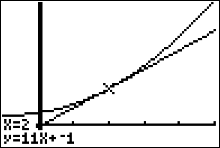
\includegraphics[width=\textwidth]{./assets/20170509-123642.png}
        \caption{A gull}
        \label{fig:gull}
    \end{subfigure}
    ~ %add desired spacing between images, e. g. ~, \quad, \qquad, \hfill etc. 
      %(or a blank line to force the subfigure onto a new line)
    \begin{subfigure}[b]{0.3\textwidth}
        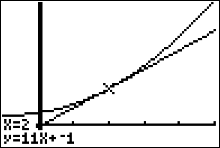
\includegraphics[width=\textwidth]{./assets/20170509-123642.png}
        \caption{A tiger}
        \label{fig:tiger}
    \end{subfigure}
    ~ %add desired spacing between images, e. g. ~, \quad, \qquad, \hfill etc. 
    %(or a blank line to force the subfigure onto a new line)
    \begin{subfigure}[b]{0.3\textwidth}
        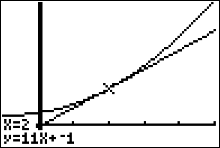
\includegraphics[width=\textwidth]{./assets/20170509-123642.png}
        \caption{A mouse}
        \label{fig:mouse}
    \end{subfigure}
    \caption{Pictures of animals}\label{fig:animals}
\end{figure}

%=-=-=-=-=-=-=-=-=-=-=-=-=-=-=-=-=-=-=-=-=-=-=-=-=-=-=-=-=-=-=-=-=-=- CHAPTER 01
\chapter{Introduction}

%=-=-=-=-=-=-=-=-=-=-=-=-=-=-=-=-=-=-=-=-=-=-=-=-=-=-=-=-=-=-=-=-=-=-=-=-=-=-=-=
% BACKMATTER
%
% Bibliographies can be prepared with BibTeX using amsplain,
% amsalpha, or (for author-year style) natbib.
%=-=-=-=-=-=-=-=-=-=-=-=-=-=-=-=-=-=-=-=-=-=-=-=-=-=-=-=-=-=-=-=-=-=-=-=-=-=-=-=

\appendix
\chapter{Appendix A}
\backmatter
\bibliographystyle{abbrv}
\bibliography{references}

%\printindex
\end{document}
%=-=-=-=-=-=-=-=-=-=-=-=-=-=-=-=-=-=-=-=-=-=-=-=-=-=-=-=-=-=-=-=-=-=-=-=-=-=-=-=
%
% END DOCUMENT
%
%=-=-=-=-=-=-=-=-=-=-=-=-=-=-=-=-=-=-=-=-=-=-=-=-=-=-=-=-=-=-=-=-=-=-=-=-=-=-=-=


%=-=-=-=-=-=-=-=-=-=-=-=-=-=-=-=-=-=-=-=-=-=-=-=-=-=-=-=-=-=-=-=-=-=-=-=-=-=-=-=
%
% GENERAL DOCUMENT STYLE GUIDE
%
% * Text should not exceed 80 characters per line to keep parsing of tex 
%   files quick.
% * 
%=-=-=-=-=-=-=-=-=-=-=-=-=-=-=-=-=-=-=-=-=-=-=-=-=-=-=-=-=-=-=-=-=-=-=-=-=-=-=-=

%=-=-=-=-=-=-=-=-=-=-=-=-=-=-=-=-=-=-=-=-=-=-=-=-=-=-=-=-=-=-=-=-=-=-=-=-=-=-=-=
% DOCUMENT STRUCTURE
%=-=-=-=-=-=-=-=-=-=-=-=-=-=-=-=-=-=-=-=-=-=-=-=-=-=-=-=-=-=-=-=-=-=-=-=-=-=-=-=
\part{}
\chapter{}
\section{}
% \subsection{}

\begin{enumerate} 
  \item something 
\end{enumerate}


% > > >  Exercises grouped in a section
\begin{xcb}
\begin{enumerate}
\item ...
\item ...
\end{enumerate}
\end{xcb}

%=-=-=-=-=-=-=-=-=-=-=-=-=-=-=-=-=-=-=-=-=-=-=-=-=-=-=-=-=-=-=-=-=-=-=-=-=-=-=-=
% FIGURES AND GRAPHICS
%
% * Figure insertion; default placement is top; if the figure occupies
%   more than 75% of a page, the [p] option should be specified.
%=-=-=-=-=-=-=-=-=-=-=-=-=-=-=-=-=-=-=-=-=-=-=-=-=-=-=-=-=-=-=-=-=-=-=-=-=-=-=-=

\begin{figure}
% \includegraphics{filename}
\caption{text of caption}
\label{}
\end{figure}

%=-=-=-=-=-=-=-=-=-=-=-=-=-=-=-=-=-=-=-=-=-=-=-=-=-=-=-=-=-=-=-=-=-=-=-=-=-=-=-=
% MATH SPECIFIC
%=-=-=-=-=-=-=-=-=-=-=-=-=-=-=-=-=-=-=-=-=-=-=-=-=-=-=-=-=-=-=-=-=-=-=-=-=-=-=-=

% > > > Numbered equation
\begin{equation}
\end{equation}

% > > > Unnumbered equation
\begin{equation*}
\end{equation*}

% > > >  Aligned equations
\begin{align}
  &  \\
  &
\end{align}

% > > >  Theorem and proof environments
\begin{theorem}[Optional addition to theorem head]
% text of theorem
\end{theorem}

\begin{proof}[Optional replacement proof heading]
% text of proof 

\end{proof}

%=+=+=+=+=+=+=+=+=+=+=+=+=+=+=+=+=+=+=+=+=+=+=+=+=+=+=+=+=+=+=+=+=+=+=+=+=+=+=+=
% END OF FILE
%=+=+=+=+=+=+=+=+=+=+=+=+=+=+=+=+=+=+=+=+=+=+=+=+=+=+=+=+=+=+=+=+=+=+=+=+=+=+=+=